\documentclass{article}
\usepackage{graphicx}
\usepackage{float}
\begin{document}
$$z^2 - az + 1 = 0$$
$$z = \frac{a \pm \sqrt{a^2 - 4}}{2}$$
\begin{figure}[H]
	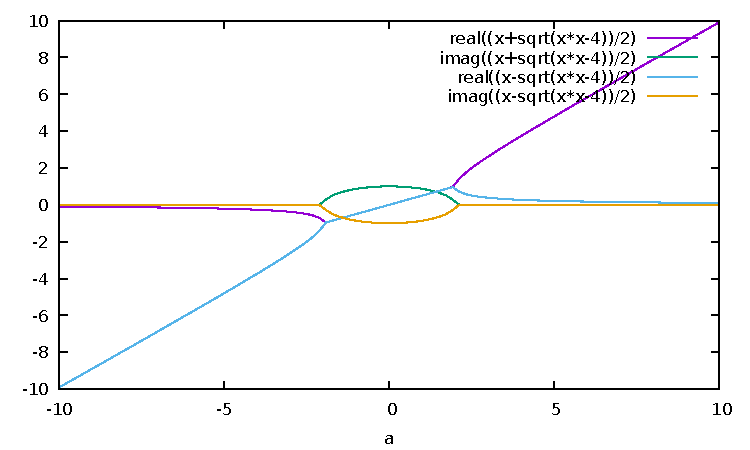
\includegraphics[width=\textwidth]{output.pdf}
\end{figure}
I intervallet <-2, 2> har ligningen komplekse løsninger. Utenfor dette intervallet er den komplekse delen av løsningene 0. 
\end{document}